	\documentclass[12pt]{book}
\usepackage[a4paper, total={6in, 8in}]{geometry}
\usepackage{amssymb}
\usepackage{listings}
\usepackage{color}
\usepackage{graphicx}
\usepackage{subfig}
\usepackage{float}
\definecolor{mygrey}{gray}{.96} % Light Grey
\definecolor{BrickRed}{RGB}{120,0,0}


\def\xbf{\mathbf{x}}
\def\zbf{\mathbf{z}}
\def\xibf{\mathbf{\xi}}
\lstset{
	language=R,              % choose the language of the code ("language=Verilog" is popular as well)
   tabsize=3,							  % sets the size of the tabs in spaces (1 Tab is replaced with 3 spaces)
	basicstyle=\footnotesize,               % the size of the fonts that are used for the code
	numbers=left,                   % where to put the line-numbers
	numberstyle=\footnotesize,              % the size of the fonts that are used for the line-numbers
	stepnumber=1,                   % the step between two line-numbers. If it's 1 each line will be numbered
	numbersep=5pt,                  % how far the line-numbers are from the code
	backgroundcolor=\color{mygrey}, % choose the background color. You must add \usepackage{color}
	showspaces=false,              % show spaces adding particular underscores
	showstringspaces=false,        % underline spaces within strings
	showtabs=false,                % show tabs within strings adding particular underscores
	frame=single,	                 % adds a frame around the code
	tabsize=3,	                    % sets default tabsize to 2 spaces
	captionpos=b,                   % sets the caption-position to bottom
	breaklines=true,                % sets automatic line breaking
	breakatwhitespace=false,        % sets if automatic breaks should only happen at whitespace
	%escapeinside={\%*}{*)},        % if you want to add a comment within your code
	commentstyle=\color{BrickRed}   % sets the comment style
}

\begin{document}
\title{\textbf{Monte Carlo Simulation Lab Assignment-7}}
\author{Yash Vanjani\\(140123046)\\Mathematics and Computing\\IIT Guwahati}
\date{March 22nd, 2016}

\maketitle

\newpage
\begin{enumerate}
\item[Q 1] Consider the multivariate normal, $X=(X_1, X_2)\thicksim N(\mu, \sum)$ where $\mu=(5, 8)$ and $\sum=(1, 2a, 2a, 4)$. For the cases $a = -0.25, 0, 0.25$, generate $1000$ values of $X$ and calculate sample means,
sample variances and sample correlations. Make empirical contour plots based on above
generated samples.
\end{enumerate}
\noindent{Code for R}

\begin{lstlisting}
library(MASS)
a<-vector("numeric")
a[1]=-0.25
a[2]=0
a[3]=0.25
u<-vector("numeric")
u[1]=5
u[2]=8
E11=1
E12=2*a
E21=2*a
E22=4
Z1<-rnorm(1000)
Z2<-rnorm(1000)
X1<-vector("numeric")
X2<-vector("numeric")
for(j in 1:3)
{	for (i in 1:1000)
	{
		X1[i]=u[1]+Z1[i]
		X2[i]=u[2]+(2*a[j]*Z1[i])+(4*Z2[i])
	}
	g<-kde2d(X1,X2)
	contour(g)
	dev.copy(png,paste(j,".png"))
	dev.off()
	cat("For a = ",a[j],"\n")
	cat("The mean of X1 is ",mean(X1),"\n")
	cat("The mean of X2 is ",mean(X2),"\n")
	cat("The variance of X1 is ",var(X1),"\n")
	cat("The variance of X2 is ",var(X2),"\n")
	cat("The covariance is ",cov(X1,X2),"\n")
	cat("The correlation is ",cor(X1,X2),"\n")
	
}
\end{lstlisting}
\newpage
\textbf{\underline{Output:}} \\\\
For $a=-0.25$:\\
\begin{lstlisting}
The mean of X1 is  4.967631 
The mean of X2 is  8.030552 
The variance of X1 is  1.02416 
The variance of X2 is  16.0848 
The covariance is  -0.6624957 
The correlation is  -0.1632268 
\end{lstlisting}
The corresponding contour plot obtained is shown below:
\begin{figure}[H]
	\centering
	\subfloat[Contour plot for $a=-0.25$]{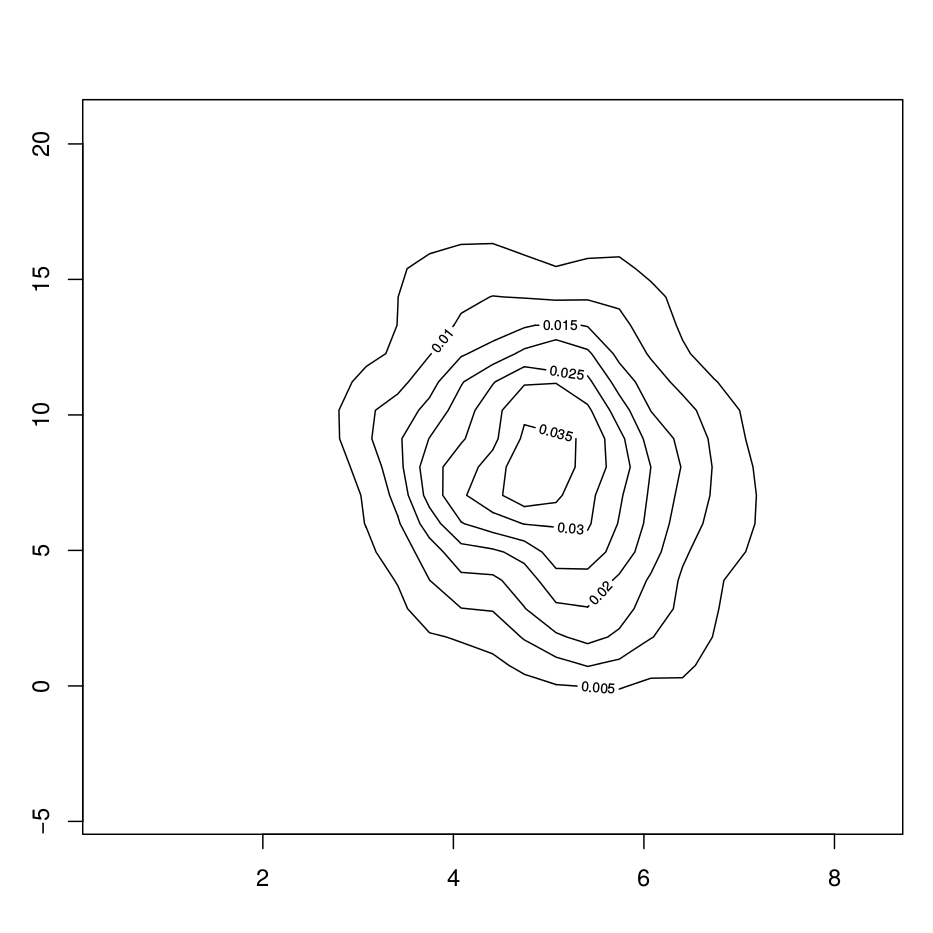
\includegraphics[width=0.6\textwidth]{q1_a=-025.png}}	
\end{figure}
\newpage
For $a=0$:
\begin{lstlisting}
The mean of X1 is  4.967631 
The mean of X2 is  8.014367 
The variance of X1 is  1.02416 
The variance of X2 is  15.67834 
The covariance is  -0.1504157 
The correlation is  -0.03753697  
\end{lstlisting}
The corresponding contour plot obtained is shown below:
\begin{figure}[H]
	\centering
	\subfloat[Contour plot for $a=0$]{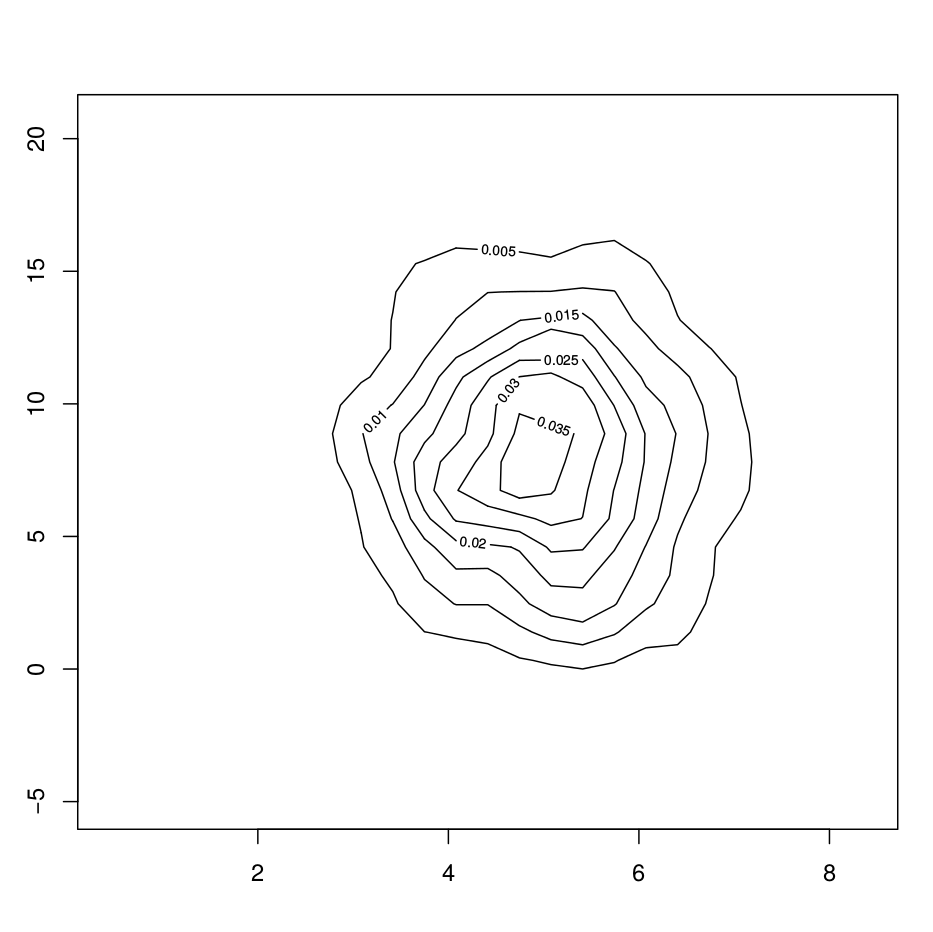
\includegraphics[width=0.6\textwidth]{q1_a=0.png}}	
\end{figure}
\newpage
For $a=0.25$:
\begin{lstlisting}
The mean of X1 is  4.967631 
The mean of X2 is  7.998183 
The variance of X1 is  1.02416 
The variance of X2 is  15.78397 
The covariance is  0.3616643 
The correlation is  0.08995259
\end{lstlisting}
The corresponding contour plot obtained is shown below:
\begin{figure}[H]
	\centering
	\subfloat[Contour plot for $a=0.25$]{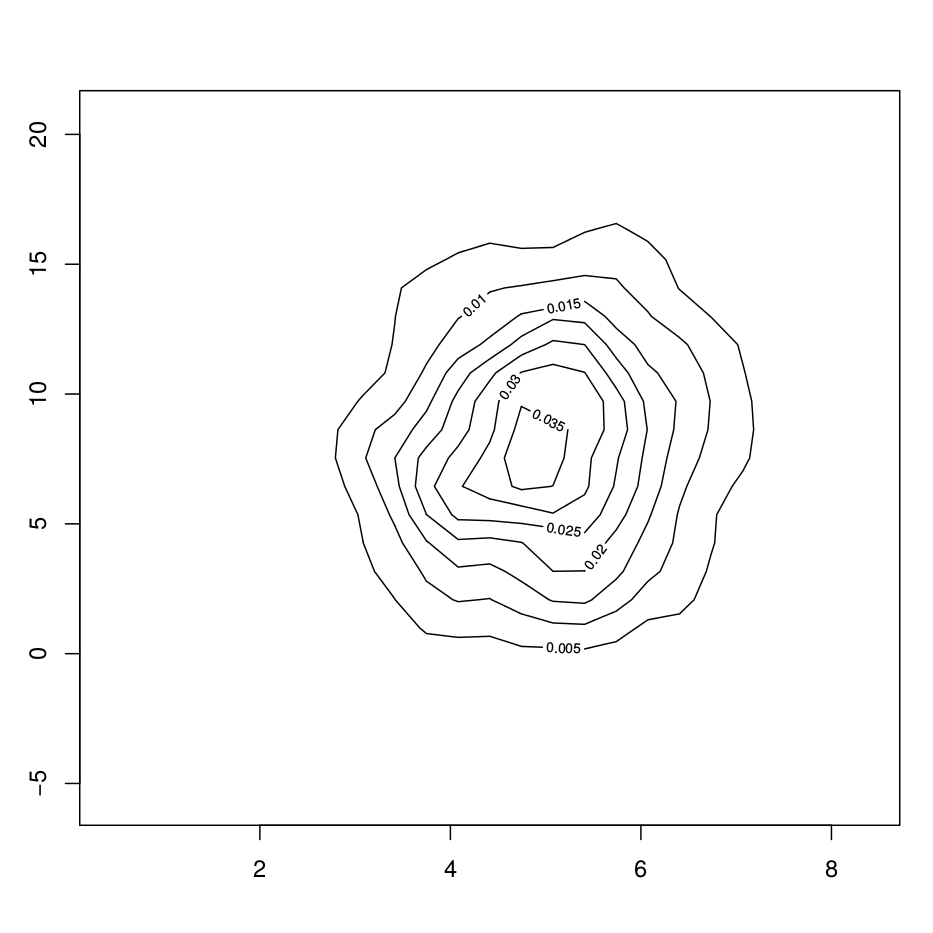
\includegraphics[width=0.6\textwidth]{q1_a=025.png}}	
\end{figure}

 

\newpage
\begin{enumerate}
\item[Q 2] Also, plot the actual and empirical marginal cdfs of $X_1$ and $X_2$ .
\end{enumerate}
\noindent{Code for R}

\begin{lstlisting}
library(MASS)
a<-vector("numeric")
a[1]=-0.25
a[2]=0
a[3]=0.25
u<-vector("numeric")
u[1]=5
u[2]=8
E11=1
E12=2*a
E21=2*a
E22=4
Z1<-rnorm(1000)
Z2<-rnorm(1000)
X1<-vector("numeric")
X2<-vector("numeric")

for (i in 1:1000)
{
	X1[i]=u[1]+Z1[i]
	X2[i]=u[2]+(2*a[1]*Z1[i])+(4*Z2[i])
}

png("X1_a=-0.25.png")
plot(ecdf(X1))
d1<-seq(0,10,length=1000)
hx<-pnorm(d1, mean=5, sd=1)
lines(d1,hx,col="red")
dev.off()

png("X2._a=-0.25png")
plot(ecdf(X2))
d2<-seq(-5,21,length=1000)
hx<-pnorm(d2, mean=8, sd=2)
lines(d2,hx,col="red")
dev.off()

for (i in 1:1000)
{
	X1[i]=u[1]+Z1[i]
	X2[i]=u[2]+(2*a[2]*Z1[i])+(4*Z2[i])
}

png("X1_a=0.png")
plot(ecdf(X1))
d1<-seq(0,10,length=1000)
hx<-pnorm(d1, mean=5, sd=1)
lines(d1,hx,col="red")
dev.off()

png("X2_a=0.png")
plot(ecdf(X2))
d2<-seq(-5,21,length=1000)
hx<-pnorm(d2, mean=8, sd=2)
lines(d2,hx,col="red")
dev.off()

for (i in 1:1000)
{
	X1[i]=u[1]+Z1[i]
	X2[i]=u[2]+(2*a[3]*Z1[i])+(4*Z2[i])
}

png("X1_a=0.25.png")
plot(ecdf(X1))
d1<-seq(0,10,length=1000)
hx<-pnorm(d1, mean=5, sd=1)
lines(d1,hx,col="red")
dev.off()

png("X2_a=0.25.png")
plot(ecdf(X2))
d2<-seq(-5,21,length=1000)
hx<-pnorm(d2, mean=8, sd=2)
lines(d2,hx,col="red")
dev.off()
}
\end{lstlisting}
\newpage
Plots of actual and emperical marginal cdfs: \\\\
Black-Empirical\\  
Red-Actual\\
\begin{figure}[H]
	\centering
	\subfloat[cdf of X1 for $a=-0.25$]{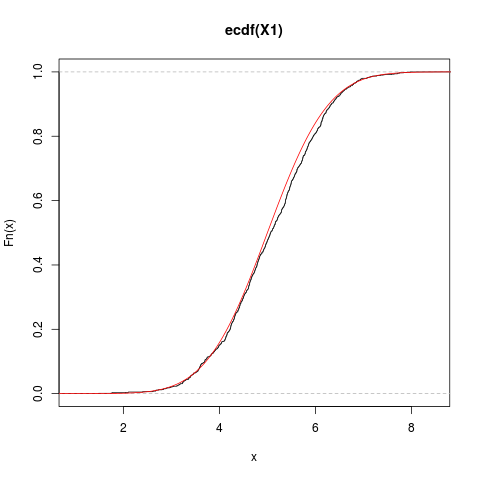
\includegraphics[width=0.5\textwidth]{X1_a=-025.png}}	
\end{figure}
\begin{figure}[H]
	\centering
	\subfloat[cdf of X2 for $a=-0.25$]{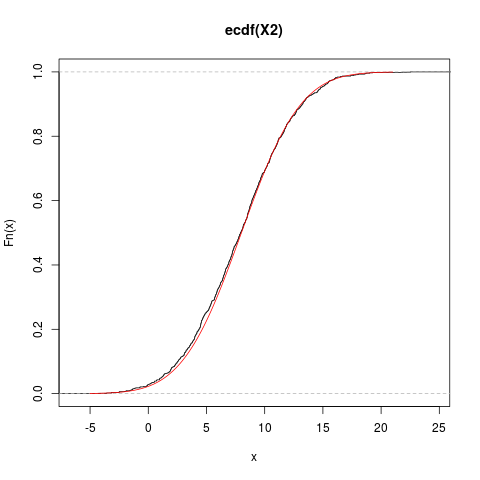
\includegraphics[width=0.5\textwidth]{X2_a=-025.png}}	
\end{figure}
 
 \begin{figure}[H]
	\centering
	\subfloat[cdf of X1 for $a=0$]{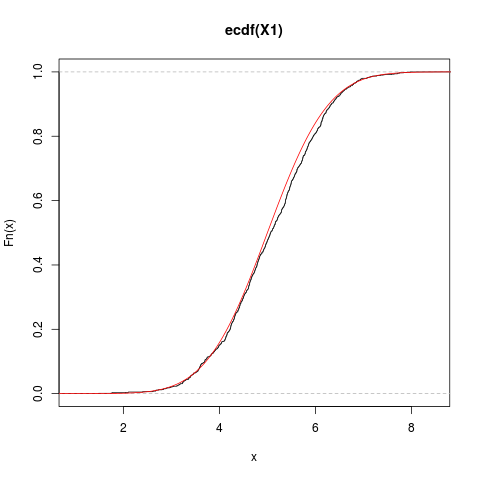
\includegraphics[width=0.6\textwidth]{X1_a=0.png}}	
\end{figure}
\begin{figure}[H]
	\centering
	\subfloat[cdf of X2 for $a=0$]{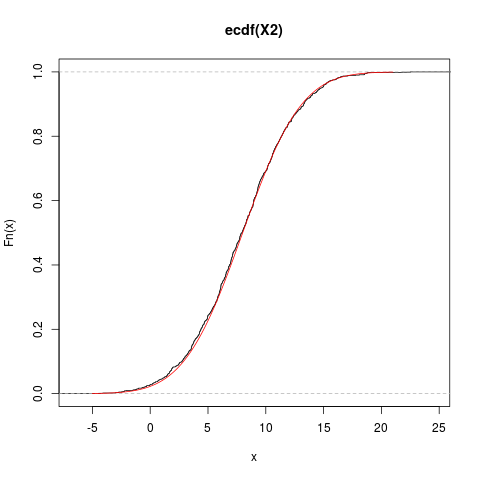
\includegraphics[width=0.6\textwidth]{X2_a=0.png}}	
\end{figure}

\begin{figure}[H]
	\centering
	\subfloat[cdf of X1 for $a=0.25$]{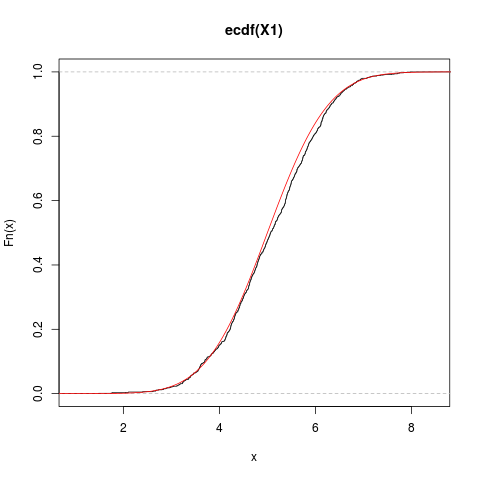
\includegraphics[width=0.6\textwidth]{X1_a=025.png}}	
\end{figure}
\begin{figure}[H]
	\centering
	\subfloat[cdf of X2 for $a=0.25$]{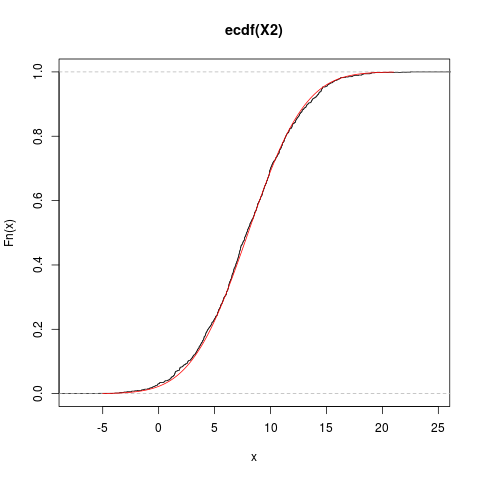
\includegraphics[width=0.6\textwidth]{X2_a=025.png}}	
\end{figure}
\newpage
\begin{enumerate}
\item[Q 3] Let us recall generating a bivariate normal with the help of conditional distributions.
Suppose that $X_1 \thicksim N (\mu_1 , {\sigma_1}^2 ), X_2 \thicksim N (\mu_2 , \sigma_2^2 )$ and the conditional distribution of
$X_2$ given $X_1 = x$ is $N (\mu_2 + \rho {\sigma_2/\sigma_1} (x - \mu_1 ), \sigma_2^2 (1 - {\rho}^2 ))$ where $|\rho| < 1$ is the correlation
coefficient between $X_1$ and $X_2$ . The vector $(X_1 , X_2 )$ is said to have a bivariate normal
distribution. Simulate the vector for a particular set of parameter values, using this
idea of conditional distributions. Estimate the sample quantities (mean, etc.) and
compare with actual values.
Take same $\mu_1 , \mu_2 , \rho_1 , \rho_2$ and $\rho$.\end{enumerate}
\noindent{Code for R}

\begin{lstlisting}
library(MASS)
a<-vector("numeric")
a[1]=-0.25
a[2]=0
a[3]=0.25
u<-vector("numeric")
u[1]=5
u[2]=8
E11=1
E12=2*a
E21=2*a
E22=4
Z1<-rnorm(1000)
Z2<-rnorm(1000)
X1<-vector("numeric")
X2<-vector("numeric")
for(j in 1:3)
{	for (i in 1:1000)
	{
		X2[i]=u[2]+(sqrt(E22)*Z2[i])
		X1[i]=(u[1]+((X2[i]-8)*a[j]/sqrt(E22)))+(Z1[i]*sqrt(1-(a[j]*a[j])))
	}
	cat("For a = ",a[j],"\n")
	cat("The mean of X1 is ",mean(X1),"\n")
	cat("The mean of X2 is ",mean(X2),"\n")
	cat("The variance of X1 is ",var(X1),"\n")
	cat("The variance of X2 is ",var(X2),"\n")
	cat("The covariance is ",cov(X1,X2),"\n")
	cat("The correlation is ",cor(X1,X2),"\n")
}
\end{lstlisting}
\newpage
The output of the code is as follows for $a=-0.25$:
\begin{lstlisting}
The mean of X1 is  4.982625 
The mean of X2 is  8.037845 
The variance of X1 is  1.020662 
The variance of X2 is  4.014131 
The covariance is  -0.5149089 
The correlation is  -0.2543862 
\end{lstlisting}

The output of the code is as follows for $a=0$:
\begin{lstlisting}
The mean of X1 is  4.986941 
The mean of X2 is  8.037845 
The variance of X1 is  1.018299 
The variance of X2 is  4.014131 
The covariance is  -0.01357344 
The correlation is  -0.006713615 
\end{lstlisting}

The output of the code is as follows for $a=0.25$:
\begin{lstlisting}
The mean of X1 is  4.992087 
The mean of X2 is  8.037845 
The variance of X1 is  1.014091 
The variance of X2 is  4.014131 
The covariance is  0.488624 
The correlation is  0.2421813 
\end{lstlisting}
\textbf{\underline{Observations:}}\\\\
1. Mean of X1 is very close to 5 as required for all values of a.\\
2. Mean of X2 is very close to 8 as required for all values of a.\\
3. Variance of X1 is very close to 1 as required for all values of a.\\
4. Variance of X2 is very close to 4 as required for all values of a.\\
5. Correlation is very close to the values required for all values of a.\\
6. Covariance is almost equal to 0 for $a=0$ as expected.
\end{document}
